%%%%%%%%%%%%%%%%%%%%%%%%%% main_referat.tex %%%%%%%%%%%%%%%%%%%%%%%%%
%
% Fisier exemplu pentru studenti 
% util in vederea redactarii de rapoarte si teme de casa
%
% Ultima editare: 6.04.2018, 
%                 Gabriela Ciuprina, gabriela.ciuprina@upb.ro
% 
% Daca aveti sugestii de imbunatatire - nu ezitati sa mi le semnalati          
%%%%%%%%%%%%%%%%%%%%%%%%%%%%%%%%%%%%%%%%%%%%%%%%%%%%%%%%%%%%%%%%%%%%%


\documentclass[12pt,twoside]{article}  % daca lucrati la o lucrare mai ampla, atunci folositi report sau book in loc de article
                                       % in cazul report sau book, prima comanda de sectionare este chapter, nu section
\usepackage{tikz}
\usepackage[siunitx]{circuitikz}
\usetikzlibrary{calc}    
\tikzset{
  dim above/.style={to path={\pgfextra{
        \pgfinterruptpath
        \draw[>=latex,|<->|] let
        \p1=($(\tikztostart)!2mm!90:(\tikztotarget)$),
        \p2=($(\tikztotarget)!2mm!-90:(\tikztostart)$)
        in(\p1) -- (\p2) node[pos=.5,sloped,above]{#1};
        \endpgfinterruptpath
      }(\tikztostart) -- (\tikztotarget) \tikztonodes
    }
  },
  dim below/.style={to path={\pgfextra{
        \pgfinterruptpath
        \draw[>=latex,|<->|] let 
        \p1=($(\tikztostart)!2mm!90:(\tikztotarget)$),
        \p2=($(\tikztotarget)!2mm!-90:(\tikztostart)$)
        in (\p1) -- (\p2) node[pos=.5,sloped,below]{#1};
        \endpgfinterruptpath
      }(\tikztostart) -- (\tikztotarget) \tikztonodes
    }
  },
}

%\usepackage{media9}
%\usepackage{animate}

\usepackage{graphicx}																		
\usepackage[romanian]{babel}
\usepackage[unicode]{hyperref} 
\usepackage{amsmath,epsfig,pifont,calc,pifont,pstricks}
\usepackage{rom} 						 % pentru a scrie cu diacritice in limba romana	
\usepackage{color}
\usepackage{listings}
\definecolor{mygreen}{RGB}{28,172,0} % color values Red, Green, Blue
\definecolor{mylilas}{RGB}{170,55,241}
\lstset{language=Matlab,%
    %basicstyle=\color{red},
    breaklines=true,%
    morekeywords={matlab2tikz},
    keywordstyle=\color{blue},%
    morekeywords=[2]{1}, keywordstyle=[2]{\color{black}},
    identifierstyle=\color{black},%
    stringstyle=\color{mylilas},
    commentstyle=\color{mygreen},%
    showstringspaces=false,%without this there will be a symbol in the places where there is a space
    numbers=left,%
    numberstyle={\tiny \color{black}},% size of the numbers
    numbersep=9pt, % this defines how far the numbers are from the text
    emph=[1]{for,end,break},emphstyle=[1]\color{red}, %some words to emphasise
    %emph=[2]{word1,word2}, emphstyle=[2]{style},    
}

	

%%% setari ale paginii
%indentarea la inceput de paragraf
\setlength{\parindent}{3ex}

%dimensiunea textului pe pagina
\setlength{\voffset}{-2cm}
\setlength{\textheight}{23cm}  
\setlength{\textwidth}{16cm}
\setlength{\topmargin}{0cm}
\setlength{\headsep}{1cm}
\renewcommand{\baselinestretch}{1.2}
\newcommand{\myindent}{\hspace*{3ex}}
%\renewcommand{\baselinestretch}{1}

%margini
\setlength{\oddsidemargin}{0.5cm}
\setlength{\evensidemargin}{-0.3cm}
%\raggedright
\raggedbottom

%% begin preambul - macro-uri definite de autor
\newcommand{\D}{\mathrm{d}}	% va fi folosita in mediul matematic, pentru diferentiala d
\newcommand{\I}{\mathrm{i}}	% va fi folosita in mediul matematic, pentru unitatea imaginara
\newcommand{\eul}{\mathrm{e}}	% numarul lui Euler
\newcommand{\vect}[1]{\mathbf{#1}}	% comanda cu un argument, pentru scrierea vectorilor cu lidere aldine, drepte
                                    % comanda \vec a LaTeX pune sageti deasupra.
																										
\newcommand{\reale}{\mbox{${\scriptstyle \rm I\!R}$}}  % multimea numerelor reale
\newcommand{\complexe}{\mbox{${\scriptstyle \rm I\!\!\!\!C}$}}
\newcommand{\rationale}{\mbox{${\scriptstyle \rm I\!\!\!\!Q}$}}
\newcommand{\naturale}{\mbox{${\scriptstyle \rm I\!\!N}$}}
\newcommand{\intregi}{\mbox{${\scriptstyle \rm Z\!\!\!Z}$}}


%% end preambul

%%%%%%%%%%%%%%%%%%%%%%%%%%%%%%%%%%%%%%%%%%%%%%%%%%%%%%%%%%%%%%%%

\begin{document}

\title{Titlu raport/tem'a\\
{\small - la disciplina *** - }}
\author{{\em Prenume Nume} \\
 Grupa, Facultate, Universitate \\
adresa de email}
\date{\today}  % sau puneti data explicit - va ramane fixata


\maketitle

%%%%%%%%%%%%%%%%%%%%%%%%%%%%%%%%%%%%%%%%%%%%%%%%%%%%%%%%%%%%%%%%%%%%%%%%%%%%%%%%%%%%%%%%%%%%%
%%%%%%%%%%%%%%%%%%                Realizator: Pop Adrian              %%%%%%%%%%%%%%%%%%%%%%%
%%%%%%%%%%%%%%%%%%%%%%%%%%%%%%%%%%%%%%%%%%%%%%%%%%%%%%%%%%%%%%%%%%%%%%%%%%%%%%%%%%%%%%%%%%%%%
\usetikzlibrary{backgrounds}
\makeatletter

%% \pgf@circ@Rlen = \pgfkeysvalueof{/tikz/circuitikz/bipoles/length}
%% Commenting the line above apparently solved the missing "Missing number, treated as zero" error

\def\TikzBipolePath#1#2{\pgf@circ@bipole@path{#1}{#2}}
\makeatother

\newlength{\ResUp} 
\newlength{\ResRight}

%%%%%%%%%%%%%%%%%%%%%%%%%%%%%%%%%%%%%%%%%%%%%%%%%%%%%%%%%%%%%%%%%%%%%%%%%%%%%%%%%%%%%%%%%%%%%
%%%%%%%%%%%%%%%%%%      Sursa de curent: simbol folosit in Romania    %%%%%%%%%%%%%%%%%%%%%%%
%%%%%%%%%%%%%%%%%%%%%%%%%%%%%%%%%%%%%%%%%%%%%%%%%%%%%%%%%%%%%%%%%%%%%%%%%%%%%%%%%%%%%%%%%%%%%
%Declaram dimensiunile initiale
\ctikzset{bipoles/romanianCurrentSource/height/.initial=.60}
\ctikzset{bipoles/romanianCurrentSource/width/.initial=.60}

%Definim noul simbol pentru SIC
\pgfcircdeclarebipole{} 
	%Offset pentru label-uri
	{\ctikzvalof{bipoles/romanianCurrentSource/height}}
	%Numele simbolului
	{romanianCurrentSource}
	%Dimensiunile "cutiei" in care va sta
	{\ctikzvalof{bipoles/romanianCurrentSource/height}}
	{\ctikzvalof{bipoles/romanianCurrentSource/width}}
	{
		%Stabilim grosimea standard a liniei pentru un element
		\pgfsetlinewidth{\pgfkeysvalueof{/tikz/circuitikz/bipoles/thickness}\pgfstartlinewidth}
		
		%Definim ancorele
		\pgfextracty{\ResUp}{\northeast}
		\pgfextractx{\ResRight}{\southwest}
		
		%Desenam cerculetul
		\pgfpathellipse{\pgfpointorigin}{\pgfpoint{0cm}{\ResUp}}{\pgfpoint{\ResRight}{0cm}}
		
		%Desenam prima sagetica; trebuie sa avem grija ca dupa ce desenam un segment,
		%urmatoarea linie va fi desenata relativ la capatul segmentului, nu fata de
		%origine, deci sunt necesare cateva repozitionari
		\pgfmoveto{\pgfpoint{1.0\ResRight}{0.0\ResUp}}   %Ne pozitionam in (-1, 0)
		\pgflineto{\pgfpoint{0.1\ResRight}{0.0\ResUp}}   %Desenam corpul sagetii
		\pgflineto{\pgfpoint{0.3\ResRight}{-0.25\ResUp}} %Desenam unul din capete
		\pgfmoveto{\pgfpoint{0.1\ResRight}{0.0\ResUp}}   %Ne pozitionam in (-0.1, 0)
	    \pgflineto{\pgfpoint{0.3\ResRight}{0.25\ResUp}}  %Desenam celalalt capat
		
		%Desenam ce-a de-a doua sagetica
		\pgfmoveto{\pgfpoint{-0.2\ResRight}{0.0\ResUp}}  %Ne pozitionam in (0.2, 0)
		\pgflineto{\pgfpoint{-1.0\ResRight}{0.0\ResUp}}  %Desenam corpul sagetii
		\pgfmoveto{\pgfpoint{0.0\ResRight}{0.25\ResUp}}  %Ne repozitionam
		\pgflineto{\pgfpoint{-0.2\ResRight}{0.0\ResUp}}  %Desenam unul din capete
		\pgflineto{\pgfpoint{0.0\ResRight}{-0.25\ResUp}} %Desenam celalat capat
		
		%Pentru desenare, sa folosim functia draw
		\pgfusepath{draw}
	}

%Ii definim un stil si o cale si...gata!
\def\romanianCurrentSourcepath#1{\TikzBipolePath{romanianCurrentSource}{#1}}
\tikzset{romanianCurrentSource/.style = {\circuitikzbasekey, /tikz/to path=\romanianCurrentSourcepath, l=#1}}


%%%%%%%%%%%%%%%%%%%%%%%%%%%%%%%%%%%%%%%%%%%%%%%%%%%%%%%%%%%%%%%%%%%%%%%%%%%%%%%%%%%%%%%%%%%%%
%%%%%%%%%%%%%%%%%%      Sursa de tensiune: simbol folosit in Romania    %%%%%%%%%%%%%%%%%%%%
%%%%%%%%%%%%%%%%%%%%%%%%%%%%%%%%%%%%%%%%%%%%%%%%%%%%%%%%%%%%%%%%%%%%%%%%%%%%%%%%%%%%%%%%%%%%%
%Declaram dimensiunile initiale
\ctikzset{bipoles/romanianVoltageSource/height/.initial=.60}
\ctikzset{bipoles/romanianVoltageSource/width/.initial=.60}

%Definim noul simbol pentru SIT
\pgfcircdeclarebipole{}
	%Stabilim grosimea standard a liniei pentru un element
	{\ctikzvalof{bipoles/romanianVoltageSource/height}}
	%Numele simbolului
	{romanianVoltageSource}
	%Dimensiunile "cutiei" in care va sta
	{\ctikzvalof{bipoles/romanianVoltageSource/height}}
	{\ctikzvalof{bipoles/romanianVoltageSource/width}}
	{
		%Stabilim grosimea standard a liniei pentru un element
		\pgfsetlinewidth{\pgfkeysvalueof{/tikz/circuitikz/bipoles/thickness}\pgfstartlinewidth}
		
		%Definim ancorele
		\pgfextracty{\ResUp}{\northeast}
		\pgfextractx{\ResRight}{\southwest}
		
		%Desenam cerculetul
		\pgfpathellipse{\pgfpointorigin}{\pgfpoint{0}{\ResUp}}{\pgfpoint{\ResRight}{0}}
		
		%Desenam prima sagetica; trebuie sa avem grija ca dupa ce desenam un segment,
		%urmatoarea linie va fi desenata relativ la capatul segmentului, nu fata de
		%origine, deci sunt necesare cateva repozitionari
		\pgfmoveto{\pgfpoint{1.0\ResRight}{0.0\ResUp}}   %Ne pozitionam in (-1, 0)
		\pgflineto{\pgfpoint{-1.0\ResRight}{0.0\ResUp}}   %Desenam corpul sagetii
		\pgflineto{\pgfpoint{-0.7\ResRight}{-0.25\ResUp}} %Desenam unul din capete
		\pgfmoveto{\pgfpoint{-1.0\ResRight}{0.0\ResUp}}   %Ne pozitionam in (-0.1, 0)
	    \pgflineto{\pgfpoint{-0.7\ResRight}{0.25\ResUp}}  %Desenam celalalt capat
		
		%Pentru desenare, sa folosim functia draw
		\pgfusepath{draw}
	}
	\def\romanianVoltageSourcepath#1{\TikzBipolePath{romanianVoltageSource}{#1}}
%Ii stabilim un nume, un posibil label si...gata!
\tikzset{romanianVoltageSource/.style = {\circuitikzbasekey, /tikz/to path=\romanianVoltageSourcepath, l=#1}}


%%%%%%%%%%%%%%%%%%%%%%%%%%%%%%%%%%%%%%%%%%%%%%%%%%%%%%%%%%%%%%%%%%%%%%%%%%%%%%%%%%%%%%%%%%%%%
%%%%%%%%%%%%%%      Sursa comandata de curent: simbol folosit in Romania    %%%%%%%%%%%%%%%%%
%%%%%%%%%%%%%%%%%%%%%%%%%%%%%%%%%%%%%%%%%%%%%%%%%%%%%%%%%%%%%%%%%%%%%%%%%%%%%%%%%%%%%%%%%%%%%
%Declaram dimensiunile initiale
\ctikzset{bipoles/romanianCCS/height/.initial=.60}
\ctikzset{bipoles/romanianCCS/width/.initial=.60}

%Definim noul simbol pentru SCC
\pgfcircdeclarebipole{} 
	%Offset pentru label-uri
	{\ctikzvalof{bipoles/romanianCCS/height}}
	%Numele simbolului
	{romanianCCS}
	%Dimensiunile "cutiei" in care va sta
	{\ctikzvalof{bipoles/romanianCCS/height}}
	{\ctikzvalof{bipoles/romanianCCS/width}}
	{
		%Stabilim grosimea standard a liniei pentru un element
		\pgfsetlinewidth{\pgfkeysvalueof{/tikz/circuitikz/bipoles/thickness}\pgfstartlinewidth}
		
		%Definim ancorele
		\pgfextracty{\ResUp}{\northeast}
		\pgfextractx{\ResRight}{\southwest}
		
		%Desenam rombul
		\pgftransformrotate{-45}
		\pgfpathrectanglecorners{\southwest}{\northeast}
		\pgftransformrotate{45}

		%Desenam prima sagetica; trebuie sa avem grija ca dupa ce desenam un segment,
		%urmatoarea linie va fi desenata relativ la capatul segmentului, nu fata de
		%origine, deci sunt necesare cateva repozitionari
		\pgfmoveto{\pgfpoint{1.25\ResRight}{0.0\ResUp}}   %Ne pozitionam in (-1, 0)
		\pgflineto{\pgfpoint{0.1\ResRight}{0.0\ResUp}}   %Desenam corpul sagetii
		\pgflineto{\pgfpoint{0.3\ResRight}{-0.25\ResUp}} %Desenam unul din capete
		\pgfmoveto{\pgfpoint{0.1\ResRight}{0.0\ResUp}}   %Ne pozitionam in (-0.1, 0)
	    \pgflineto{\pgfpoint{0.3\ResRight}{0.25\ResUp}}  %Desenam celalalt capat
		
		%Desenam ce-a de-a doua sagetica
		\pgfmoveto{\pgfpoint{-0.2\ResRight}{0.0\ResUp}}  %Ne pozitionam in (0.2, 0)
		\pgflineto{\pgfpoint{-1.25\ResRight}{0.0\ResUp}}  %Desenam corpul sagetii
		\pgfmoveto{\pgfpoint{0.0\ResRight}{0.25\ResUp}}  %Ne repozitionam
		\pgflineto{\pgfpoint{-0.2\ResRight}{0.0\ResUp}}  %Desenam unul din capete
		\pgflineto{\pgfpoint{0.0\ResRight}{-0.25\ResUp}} %Desenam celalat capat
		
		%Pentru desenare, sa folosim functia draw
		\pgfusepath{draw}
	}

%Ii definim un stil si o cale si...gata!
\def\romanianCCS#1{\TikzBipolePath{romanianCCS}{#1}}
\tikzset{romanianCCS/.style = {\circuitikzbasekey, /tikz/to path=\romanianCCS, l=#1}}


%%%%%%%%%%%%%%%%%%%%%%%%%%%%%%%%%%%%%%%%%%%%%%%%%%%%%%%%%%%%%%%%%%%%%%%%%%%%%%%%%%%%%%%%%%%%%
%%%%%%%%%%%%%      Sursa comandata de tensiune: simbol folosit in Romania    %%%%%%%%%%%%%%%%
%%%%%%%%%%%%%%%%%%%%%%%%%%%%%%%%%%%%%%%%%%%%%%%%%%%%%%%%%%%%%%%%%%%%%%%%%%%%%%%%%%%%%%%%%%%%%
%Declaram dimensiunile initiale
\ctikzset{bipoles/romanianCVS/height/.initial=.60}
\ctikzset{bipoles/romanianCVS/width/.initial=.60}

%Definim noul simbol pentru CVS
\pgfcircdeclarebipole{}
	%Stabilim grosimea standard a liniei pentru un element
	{\ctikzvalof{bipoles/romanianCVS/height}}
	%Numele simbolului
	{romanianCVS}
	%Dimensiunile "cutiei" in care va sta
	{\ctikzvalof{bipoles/romanianCVS/height}}
	{\ctikzvalof{bipoles/romanianCVS/width}}
	{
		%Stabilim grosimea standard a liniei pentru un element
		\pgfsetlinewidth{\pgfkeysvalueof{/tikz/circuitikz/bipoles/thickness}\pgfstartlinewidth}
		
		%Definim ancorele
		\pgfextracty{\ResUp}{\northeast}
		\pgfextractx{\ResRight}{\southwest}
		
		%Desenam rombul
		\pgftransformrotate{-45}
		\pgfpathrectanglecorners{\southwest}{\northeast}
		\pgftransformrotate{45}
		
		%Desenam prima sagetica; trebuie sa avem grija ca dupa ce desenam un segment,
		%urmatoarea linie va fi desenata relativ la capatul segmentului, nu fata de
		%origine, deci sunt necesare cateva repozitionari
		\pgfmoveto{\pgfpoint{1.25\ResRight}{0.0\ResUp}}   %Ne pozitionam in (-1.25, 0)
		\pgflineto{\pgfpoint{-1.3\ResRight}{0.0\ResUp}}  %Desenam corpul sagetii
		\pgflineto{\pgfpoint{-0.9\ResRight}{-0.25\ResUp}} %Desenam unul din capete
		\pgfmoveto{\pgfpoint{-1.3\ResRight}{0.0\ResUp}}   %Ne pozitionam in (-0.1, 0)
	    \pgflineto{\pgfpoint{-0.9\ResRight}{0.25\ResUp}}  %Desenam celalalt capat
		
		%Pentru desenare, sa folosim functia draw
		\pgfusepath{draw}
	}
	\def\romanianCVS#1{\TikzBipolePath{romanianCVS}{#1}}
%Ii stabilim un nume, un posibil label si...gata!
\tikzset{romanianCVS/.style = {\circuitikzbasekey, /tikz/to path=\romanianCVS, l=#1}}


%%%%%%%%%%%%%%%%%%%%%%%%%%%%%%%%%%%%%%%%%%%%%%%%%%%%%%%%%%%%%%%%%%%%%%%%%%%%%%%%%%%%%%%%%%%%%
%%%%%%%%%%%%%%%%%      Dioda Zenner 1 & 2: simbol folosit in Romania    %%%%%%%%%%%%%%%%%%%%%
%%%%%%%%%%%%%%%%%%%%%%%%%%%%%%%%%%%%%%%%%%%%%%%%%%%%%%%%%%%%%%%%%%%%%%%%%%%%%%%%%%%%%%%%%%%%%
%Declaram dimensiunile initiale
\ctikzset{bipoles/zDoZ/height/.initial=.60}
\ctikzset{bipoles/zDoZ/width/.initial=1.00}
  
%Definim noul simbol pentru diodaZenner
\pgfcircdeclarebipole{}
	%Stabilim grosimea standard a liniei pentru un element
	{\ctikzvalof{bipoles/zDoZ/height}}
	%Numele simbolului
	{zDoZ}
	%Dimensiunile "cutiei" in care va sta
	{\ctikzvalof{bipoles/zDoZ/height}}
	{\ctikzvalof{bipoles/zDoZ/width}}
	{
		%Stabilim grosimea standard a liniei pentru un element
		\pgfsetlinewidth{\pgfkeysvalueof{/tikz/circuitikz/bipoles/thickness}\pgfstartlinewidth}
		
		%Definim ancorele
		\pgfextracty{\ResUp}{\northeast}
		\pgfextractx{\ResRight}{\southwest}
		
		%Desenam, fara alte explicatii, ca acum stim
		\pgfmoveto{\pgfpoint{0.0\ResRight}{0.0\ResUp}}
		\pgflineto{\pgfpoint{1.0\ResRight}{0.6\ResUp}}
		\pgflineto{\pgfpoint{1.0\ResRight}{-0.6\ResUp}}
		\pgflineto{\pgfpoint{-1.0\ResRight}{0.6\ResUp}}
		\pgflineto{\pgfpoint{-1.0\ResRight}{-0.6\ResUp}}
		
		%Pentru desenare, sa folosim functia draw
		\pgfusepath{draw}
	}
	\def\zDoZ#1{\TikzBipolePath{zDoZ}{#1}}
%Ii stabilim un nume, un posibil label si...gata!
\tikzset{zDoZ/.style = {\circuitikzbasekey, /tikz/to path=\zDoZ, l=#1}}


%Declaram dimensiunile initiale
\ctikzset{bipoles/zDoZZ/height/.initial=.60}
\ctikzset{bipoles/zDoZZ/width/.initial=1.00}
  
%Definim noul simbol pentru diodaZennerInversa
\pgfcircdeclarebipole{}
	%Stabilim grosimea standard a liniei pentru un element
	{\ctikzvalof{bipoles/zDoZZ/height}}
	%Numele simbolului
	{zDoZZ}
	%Dimensiunile "cutiei" in care va sta
	{\ctikzvalof{bipoles/zDoZZ/height}}
	{\ctikzvalof{bipoles/zDoZZ/width}}
	{
		%Stabilim grosimea standard a liniei pentru un element
		\pgfsetlinewidth{\pgfkeysvalueof{/tikz/circuitikz/bipoles/thickness}\pgfstartlinewidth}
		
		%Definim ancorele
		\pgfextracty{\ResUp}{\northeast}
		\pgfextractx{\ResRight}{\southwest}
		
		%Desenam, fara alte explicatii, ca acum stim
		\pgfmoveto{\pgfpoint{0.0\ResRight}{0.0\ResUp}}
		\pgflineto{\pgfpoint{1.0\ResRight}{-0.6\ResUp}}
		\pgflineto{\pgfpoint{1.0\ResRight}{0.6\ResUp}}
		\pgflineto{\pgfpoint{-1.0\ResRight}{-0.6\ResUp}}
		\pgflineto{\pgfpoint{-1.0\ResRight}{0.6\ResUp}}
		
		%Pentru desenare, sa folosim functia draw
		\pgfusepath{draw}
	}
	\def\zDoZZ#1{\TikzBipolePath{zDoZZ}{#1}}
%Ii stabilim un nume, un posibil label si...gata!
\tikzset{zDoZZ/.style = {\circuitikzbasekey, /tikz/to path=\zDoZZ, l=#1}}


%%%%%%%%%%%%%%%%%%%%%%%%%%%%%%%%%%%%%%%%%%%%%%%%%%%%%%%%%%%%%%%%%%%%%%%%%%%%%%%%%%%%%%%%%%%%%
%%%%%%%%%%%%%%%%      Condensator neliniar: simbol folosit in Romania    %%%%%%%%%%%%%%%%%%%%
%%%%%%%%%%%%%%%%%%%%%%%%%%%%%%%%%%%%%%%%%%%%%%%%%%%%%%%%%%%%%%%%%%%%%%%%%%%%%%%%%%%%%%%%%%%%%
%Declaram dimensiunile initiale
\ctikzset{bipoles/Cn/height/.initial=.40}
\ctikzset{bipoles/Cn/width/.initial=1.00}

%Definim noul simbol pentru condNeliniar
\pgfcircdeclarebipole{}
	%Stabilim grosimea standard a liniei pentru un element
	{\ctikzvalof{bipoles/Cn/height}}
	%Numele simbolului
	{Cn}
	%Dimensiunile "cutiei" in care va sta
	{\ctikzvalof{bipoles/Cn/height}}
	{\ctikzvalof{bipoles/Cn/width}}
	{
		%Stabilim grosimea standard a liniei pentru un element
		\pgfsetlinewidth{\pgfkeysvalueof{/tikz/circuitikz/bipoles/thickness}\pgfstartlinewidth}
		
		%Definim ancorele
		\pgfextracty{\ResUp}{\northeast}
		\pgfextractx{\ResRight}{\southwest}
		
		%Desenam dreptunghiul
		\pgfpathrectanglecorners{\southwest}{\northeast}
		
		%Desenam cele doua linii paralele
		\pgfmoveto{\pgfpoint{0.2\ResRight}{0.8\ResUp}}
		\pgflineto{\pgfpoint{0.2\ResRight}{-0.8\ResUp}}
		
		\pgfmoveto{\pgfpoint{-0.2\ResRight}{0.8\ResUp}}
		\pgflineto{\pgfpoint{-0.2\ResRight}{-0.8\ResUp}}
		
		%Desenam liniile de pe mijloc
		\pgfmoveto{\pgfpoint{1.0\ResRight}{0.0\ResUp}}
		\pgflineto{\pgfpoint{0.2\ResRight}{0.0\ResUp}}
		
		\pgfmoveto{\pgfpoint{-0.2\ResRight}{0.0\ResUp}}
		\pgflineto{\pgfpoint{-1.0\ResRight}{0.0\ResUp}}
		
		%Pentru desenare, sa folosim functia draw
		\pgfusepath{draw}
		
		%Desenam chestiuta neagra
		\pgfsetlinewidth{5.0\pgfkeysvalueof{/tikz/circuitikz/bipoles/thickness}\pgfstartlinewidth}
		\pgfmoveto{\pgfpoint{-1.0\ResRight}{1.0\ResUp}}
		\pgflineto{\pgfpoint{-1.0\ResRight}{-1.0\ResUp}}
		\pgfmoveto{\pgfpoint{-0.9\ResRight}{1.0\ResUp}}
		\pgflineto{\pgfpoint{-0.9\ResRight}{-1.0\ResUp}}
		\pgfmoveto{\pgfpoint{-0.8\ResRight}{1.0\ResUp}}
		\pgflineto{\pgfpoint{-0.8\ResRight}{-1.0\ResUp}}
		
		%Pentru desenare, sa folosim functia draw
		\pgfusepath{draw}
	}
	\def\Cn#1{\TikzBipolePath{Cn}{#1}}
%Ii stabilim un nume, un posibil label si...gata!
\tikzset{Cn/.style = {\circuitikzbasekey, /tikz/to path=\Cn, l=#1}}


%%%%%%%%%%%%%%%%%%%%%%%%%%%%%%%%%%%%%%%%%%%%%%%%%%%%%%%%%%%%%%%%%%%%%%%%%%%%%%%%%%%%%%%%%%%%%
%%%%%%%%%%%%%%%%%%      Bobina neliniara: simbol folosit in Romania    %%%%%%%%%%%%%%%%%%%%%%
%%%%%%%%%%%%%%%%%%%%%%%%%%%%%%%%%%%%%%%%%%%%%%%%%%%%%%%%%%%%%%%%%%%%%%%%%%%%%%%%%%%%%%%%%%%%%
%Declaram dimensiunile initiale
\ctikzset{bipoles/Ln/height/.initial=.40}
\ctikzset{bipoles/Ln/width/.initial=1.00}

%Definim noul simbol pentru condNeliniar
\pgfcircdeclarebipole{}
	%Stabilim grosimea standard a liniei pentru un element
	{\ctikzvalof{bipoles/Ln/height}}
	%Numele simbolului
	{Ln}
	%Dimensiunile "cutiei" in care va sta
	{\ctikzvalof{bipoles/Ln/height}}
	{\ctikzvalof{bipoles/Ln/width}}
	{
		%Stabilim grosimea standard a liniei pentru un element
		\pgfsetlinewidth{\pgfkeysvalueof{/tikz/circuitikz/bipoles/thickness}\pgfstartlinewidth}
		
		%Definim ancorele
		\pgfextracty{\ResUp}{\northeast}
		\pgfextractx{\ResRight}{\southwest}
		
		%Desenam dreptunghiul
		\pgfpathrectanglecorners{\southwest}{\northeast}
	
		%Desenam spirele
		\pgfmoveto{\pgfpoint{1.0\ResRight}{0.0\ResUp}}
		\pgflineto{\pgfpoint{0.80\ResRight}{0.0\ResUp}}
		\pgfpatharc{0}{-180}{\ResRight/6}
		\pgfpatharc{0}{-180}{\ResRight/6}
		\pgfpatharc{0}{-180}{\ResRight/6}
		\pgfpatharc{0}{-180}{\ResRight/6}
		\pgflineto{\pgfpoint{-0.8\ResRight}{0.0\ResUp}}
		
		%Pentru desenare, sa folosim functia draw
		\pgfusepath{draw}
		
		%Desenam chestiuta neagra
		\pgfsetlinewidth{5.3\pgfkeysvalueof{/tikz/circuitikz/bipoles/thickness}\pgfstartlinewidth}
		\pgfmoveto{\pgfpoint{-1.0\ResRight}{1.0\ResUp}}
		\pgflineto{\pgfpoint{-1.0\ResRight}{-1.0\ResUp}}
		\pgfmoveto{\pgfpoint{-0.9\ResRight}{1.0\ResUp}}
		\pgflineto{\pgfpoint{-0.9\ResRight}{-1.0\ResUp}}
		\pgfmoveto{\pgfpoint{-0.8\ResRight}{1.0\ResUp}}
		\pgflineto{\pgfpoint{-0.8\ResRight}{-1.0\ResUp}}

		
		%Pentru desenare, sa folosim functia draw
		\pgfusepath{draw}
	}
	\def\Ln#1{\TikzBipolePath{Ln}{#1}}
%Ii stabilim un nume, un posibil label si...gata!
\tikzset{Ln/.style = {\circuitikzbasekey, /tikz/to path=\Ln, l=#1}}




\paragraph{Abstract}
Acest document 'si pachetul de fi'siere asociat sunt utile studen'tilor care doresc s'a 'i'si tehnoredacteze rapoartele de cercetare, referatele de laborator sau temele de cas'a 'in \LaTeX. El este rezultatul compil'arii fi'sierelor surs'a pe care le g'asi'ti la adresa
{\href{http://www.lmn.pub.ro/~gabriela/LatexTemplate4Students}{http://www.lmn.pub.ro/$\sim$gabriela/LatexTemplate4Students}}. Simultan cu citirea lui, trebuie s'a urm'ari'ti 'si con'tinutul fi'sierelor surs'a, 'in care au fost comentate c\^ateva detalii utile. Urm'ari'ti 'in acest document doar indica'tiile de redactare 'si exemplele. Acest document nu are niciun fel de con'tinut 'stiin'tific.
Dac'a ave'ti 'intreb'ari sau sugestii de 'imbun'at'a'tire a acestei machete, sunte'ti ruga'ti s'a le semnala'ti la
\texttt{gabriela.ciuprina@upb.ro}. 

Detalii despre \LaTeX\ g'asi'ti pe net, pute'ti 'incepe de la 
{\href{http://www.latex-project.org/}{http://www.latex-project.org/}}.

Este bine ca orice raport s'a aib'a un abstract de aproximativ 10 r\^anduri din care s'a se 'in'teleag'a ce con'tine documentul 'si care este contribu'tia cea mai important'a adus'a.


%%% Odata ce v-ati definit fisierul principal, incluzand preambulul si macro-urile, nu trebuie decat sa va concentrati pe fond
%%% Succes la scris!

\vspace*{3cm}
{\color{blue}
\em
\hfill "Writing is thinking. To write well is to think clearly. That$'$s why it$'$s so hard."  % din cauza lui rom.sty care a modificat ' pentru diacritice

\hfill ― David McCullough
}

% generarea automata a cuprinsului
\newpage  % cuprinsul pus pe pagina noua
\tableofcontents
\newpage  % continutul propriu-zis sa inceapa pe pagina noua

\renewcommand\tablename{Tabelul}  % altfel scrie "Tabela"
\renewcommand\bibname{Referin'te}  % altfel scrie "Bibliografie" si acum referintele includ si pagini web

%%%%%%%%% continutul propriu zis al lucrarii
% Daca documentul e mare, este bine atunci sa il impartiti in mai multe fisiere (si eventual mai multe foldere)
\section{Redactarea 'in \LaTeX. C\^ateva sfaturi generale}
\label{sec:general}
% \label{nume} - este o eticheta pusa in contexul ultimei numerotari, in acest caz este numarul sectiunii.
% Pentru a va referi la ea, va trebui sa folositi \ref{nume}
%
% Este recomandat ca numele referintei sa indice tipul de referinta (in exemplul de mai sus, este o sectiune)


'In \LaTeX\ pute'ti redacta  rapoarte 'stiin'tifice care s'a arate impecabil. Pentru a v'a ini'tia 'in folosirea \LaTeX\ v'a recomand s'a citi'ti de exemplu un tutorial cum ar fi
{\em LaTeX Tutorial}, disponibil la 
\href{http://ece.uprm.edu/~caceros/latex/introduction.pdf}{http://ece.uprm.edu/$~$caceros/latex/introduction.pdf} 'si s'a ave'ti la 'indem\^an'a o carte mai detaliat'a, cum ar fi
{\em The Not So Short Introduction to Latex}, disponibil'a la
\href{https://tobi.oetiker.ch/lshort/lshort.pdf}{https://tobi.oetiker.ch/lshort/lshort.pdf}. 
Dac'a nu parcurge'ti o astfel de documenta'tie, atunci frazele de mai jos s-ar putea s'a va apar'a ca fiind f'ar'a sens.


\subsection{Structurarea documentului}
\label{sec:structura}
'Inainte de a scrie un raport, trebuie s'a stabili'ti cuprinsul lui. 
Dup'a fiecare comand'a de sec'tionare, scrie'ti un scurt paragraf explicativ pentru ce urmeaz'a.

\LaTeX\ ofer'a multe comenzi 'si macro-uri, dar pot fi definite 'si  unele noi. 
Este recomandat ca toate macro-urile noi definite s'a fie puse 'in preambul
('intre ultima comand'a \texttt{\string\usepackage} 'si
\texttt{\string\begin\string{document\string}}). Remarca'ti macro-urile noi definite pentru generarea acestui document ('in fi'sierul 
principal, \texttt{\string\newcommand}).

Folosi'ti automatismul \LaTeX\  pentru a face referin'te 'incruci'sate c'atre numere de sec'tiuni, ecua'tii, figuri.
Detalii g'asi'ti 'in documenta'tia recomandat'a la 'inceputul paragraful \ref{sec:general}.

Etichetele trebuie s'a fie unice, altfel la compilarea fi'sierelor vor apare {\em warnings}, iar rezultatul va avea referin'te nerezolvate, marcate cu \texttt{[?]}. {\color{red} Pentru un rezultat impecabil trebuie s'a ave'ti 
\texttt{0 Error(s), 0 Warning(s)}}.


\subsection{C\^ateva detalii}
\label{sec:detalii} 
Urmeaz'a c\^ateva detalii, despre modul de scriere al ecua'tiilor, inserare a figurilor 'si tabelelor.

\subsubsection{Ecua'tii}
Ecua'tiile sunt centrate. Vectorii se noteaz'a cu litere aldine, drepte, ca de exemplu
%                                        % nu lasati un rand liber intre text si ecuatia care continua fraza
\begin{equation}
\label{eq:produs_vectorial}
\vect{a}\times\vect{b}=\vect{c},          % se folosesc semne de punctuatie 'si in ecua'tie; aici se termina propozitia
\end{equation}
unde $\vect{a}$, $\vect{b}$, $\vect{c}$ sunt vectori reali $n$ dimensionali.

Referirea la ecua'tii se face dup'a cum urmeaz'a:
\begin{itemize}
\item Rela'tia (\ref{eq:produs_vectorial}) noteaz'a produsul vectorial dintre vectorii $\vect{a}$ 'si $\vect{b}$ cu $\vect{c}$.
\item Dar, observa'ti c'a 'in (\ref{eq:produs_vectorial}) produsul vectorial este notat cu $\times$.
\end{itemize}
'In concluzie, 'incepe'ti o propozi'tie cu cuv\^antul ``Rela'tia" sau  ``Ecua'tia" dar  nu folosi'ti cuv\^antul ``ecua'tia"
sau abrevierea  ``ec." atunci c\^and referin'ta este 'in mijlocul frazei.

Folosi'ti ``$\times$"  pentru a indica un produs vectorial, 'si ,
``$\cdot$" pentru a indica un produs scalar. La 'inmul'tirea dintre un scalar 'si un vector nu pune'ti punct, de exemplu
\begin{equation}
\label{eq:produs_scalar_vector}
\vect{y} = \alpha \vect{a},           % litere grecesti \alpha \beta \gamma \delta \Delta \omega \Omega \varphi   etc
\end{equation}
unde $\alpha \in \reale$ este un scalar real, iar $\vect{a}, \vect{y} \in \reale^n$. 'Intotdeauna trebuie s'a existe 'in text explica'tiile m'arimilor care intervin 'in rela'tiile matematice.

Indicii 'si puterile trebuie s'a fie scrise cu litere drepte atunci c\^and sunt cuvinte sau abrevieri.
De asemenea, unit'a'tile de m'asur'a, operatorii diferen'tiali 'si unitatea imaginar'a trebuie scrise cu litere drepte, ca de exemplu:
\begin{equation}
V_{\mathrm{out}} = \oint_C \vect{E}\cdot\D \vect{r} = -\frac{\D\varphi}{\D t} =  % \D este definita in preambul
4.7\,\mu\mathrm{V},
% "\," de mai sus adauga un mic spatiu intre valoare si unitatea de masura 
\end{equation}
sau
\begin{equation}
\label{eq:nabla}
\nabla\times\vect{E} = -\I \omega\mu\vect{H}.
\end{equation}
Observa'ti micul spa'tiu dintre num'ar 'si unitatea de m'asur'a. Folosi'ti
``$\varDelta$" pentru un increment infinitezimal 'si ``$\eul$" pentru num'arul lui Euler.  %\eul a fost definit in preambul
Observa'ti modul de folosire a semnelor de punctua'tie. Nu l'asa'ti r\^anduri libere 'in fi'sierele \texttt{.tex} dec\^at atunci c\^and 'incepe un paragraf nou, altfel documentul va fi pres'arat cu o mul'time de spa'tii goale. Observa'ti c'a 'in fi'sierul surs'a, dup'a ecua'tia
(\ref{eq:nabla}) nu exist'a niciun r\^and liber, iar paragraful urm'ator este, 'in consecin't'a, neindentat.

Nu folosi'ti trecerea for'tat'a la r\^and nou, cu \verb \\  dec\^at 'in situa'tii excep'tionale!

Dac'a ave'ti mai multe ecua'tii de aliniat una sub alta pute'ti folosi \texttt{eqnarray}, caz 'in care rezultatul arat'a astfel
\begin{eqnarray}
x & = & \frac{y}{z}, \\
z & = & \sum_{i=1}^n a_k,
\end{eqnarray}
sau \texttt{equation} combinat cu \texttt{array} caz 'in care rezultatul arat'a mai compact, astfel:
\begin{equation}
\begin{array}{ccl} % c - centrat, l - aliniat la stanga
x & = & \frac{y}{z}, \\
z & = & \sum_{i=1}^n a_k.
\end{array}
\end{equation}
'In primul caz toate ecua'tiile sunt numerotate dac'a nu exist'a o instruc'tiune special'a \texttt{\string\nonumber} care s'a anuleze numerotarea. 'In al doilea caz, grupul de rela'tii va avea un singur num'ar. Al doilea caz permite 'si marcarea grupului cu acolade, ca 'in exemplul urm'ator, 'in care a fost blocat'a 'si numerotarea automat'a.
\begin{equation}
\left\{
\begin{array}{ccl} % c - centrat, l - aliniat la stanga
x & = & \frac{y}{z}, \\
z & = & \sum_{i=1}^n a_k.
\end{array}  
\right. \nonumber % marcarea inchiderii - falsa; blocarea numerotarii
\end{equation}

\subsubsection{Figuri}

Figurile trebuie s'a arate ca 'in Fig.~\ref{fig:figura_exemplu}. Referirea la figuri se face astfel:
\begin{itemize}
\item Figura \ref{fig:figura_exemplu} $\ldots$ atunci c\^and propozi'tia 'incepe cu cuv\^antul
``Figura".
\item 'In mijlocul unei propozi'tii, se scrie "'in Fig.~\ref{fig:figura_exemplu} pute'ti observa ....".
\end{itemize}

\begin{figure}[ht]  %preferinte: mai intai h - here apoi t- top, htb-, b-bottom
\centering
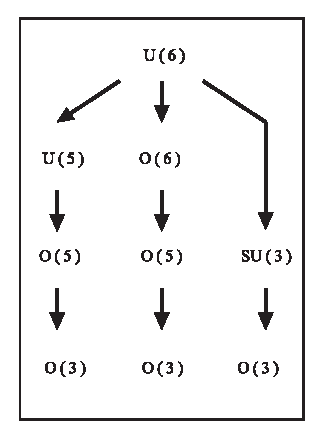
\includegraphics{tex_files/figs/authorfig1.eps}
%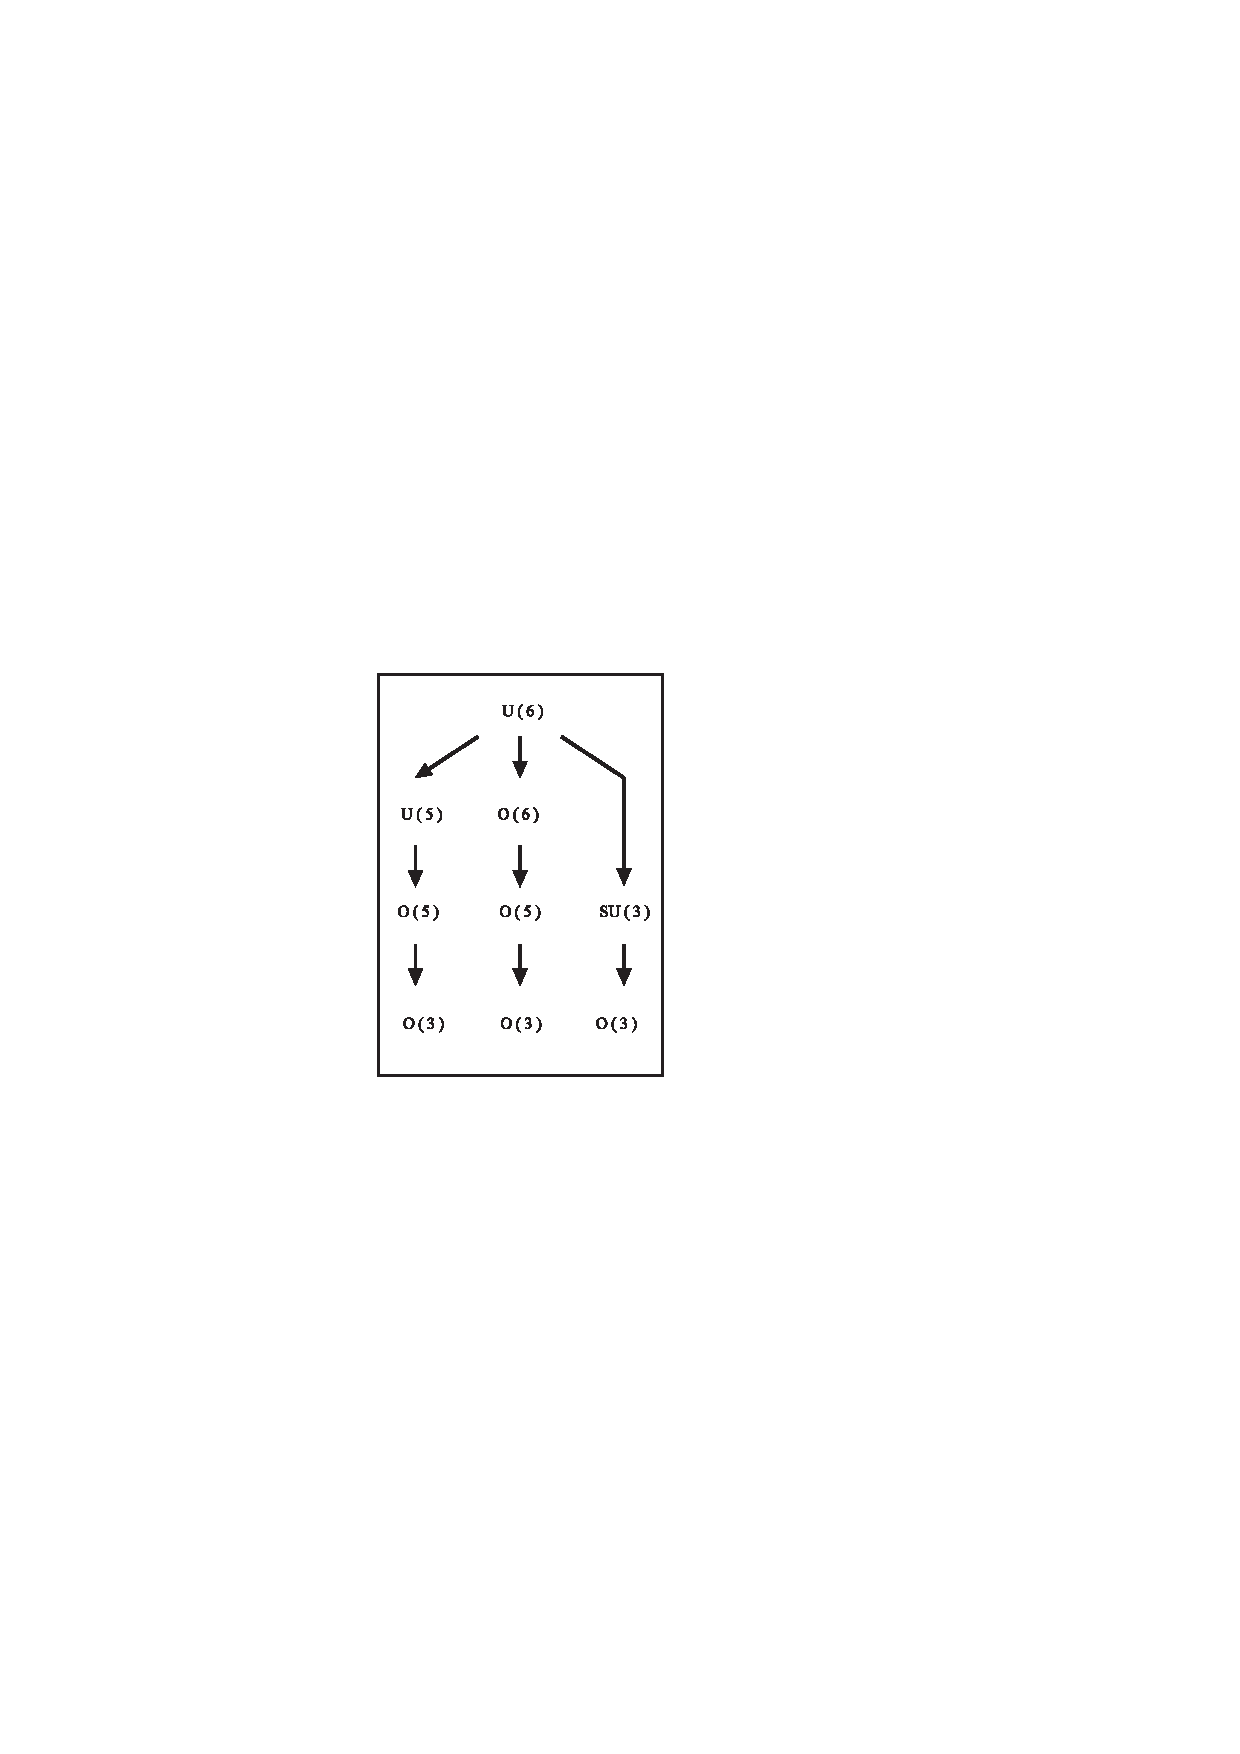
\includegraphics{tex_files/figs/authorfig1.jpeg}
\caption{O figur'a are 'intotdeauna un titlu scris sub ea, iar 'in text exist'a o referire la ea. G'asi'ti 'in text referirea la aceast'a figur'a.}
\label{fig:figura_exemplu}       
\end{figure}

Dac'a este necesar, pute'ti pune dou'a figuri una l\^ang'a alta, fie cu un titlu comun ca 'in Fig.\ref{fig:figura_exemplu2}, fie cu titluri separate ca 'in Fig.\ref{fig:figura_exemplu3} 'si Fig.\ref{fig:figura_exemplu4}. Titlurile au semne de punctua'tie!
\begin{figure}[ht]  %h - here, dar puteti pune si t-top, b-bottom
\begin{minipage}{0.5\textwidth}
\centering
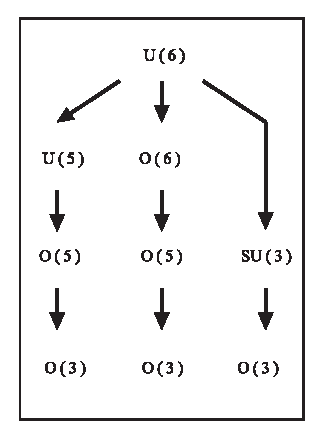
\includegraphics{tex_files/figs/authorfig1.eps}
%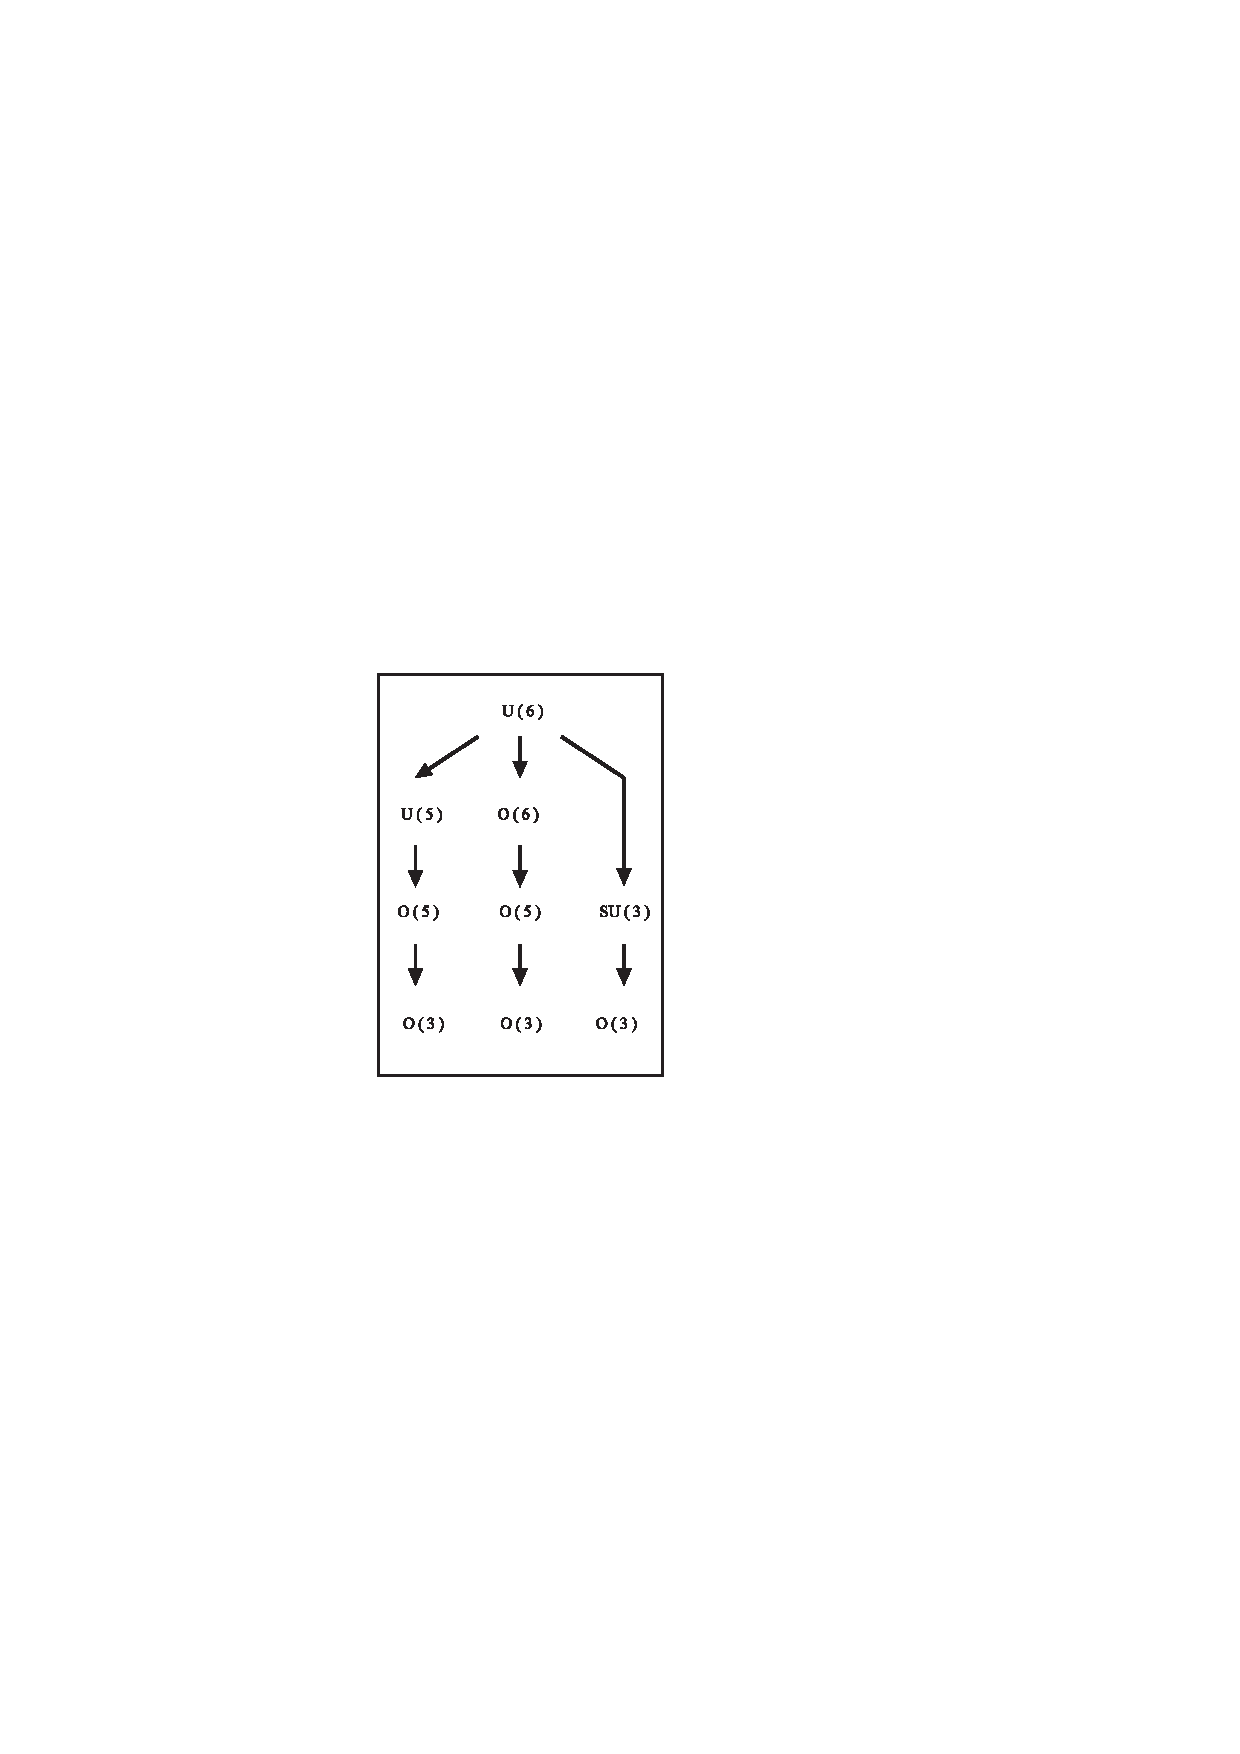
\includegraphics{tex_files/figs/authorfig1.jpeg}
\end{minipage}
\begin{minipage}{0.5\textwidth}
\centering
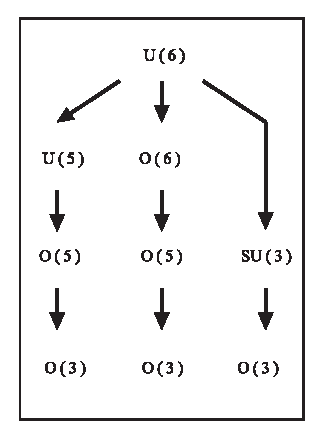
\includegraphics{tex_files/figs/authorfig1.eps}
%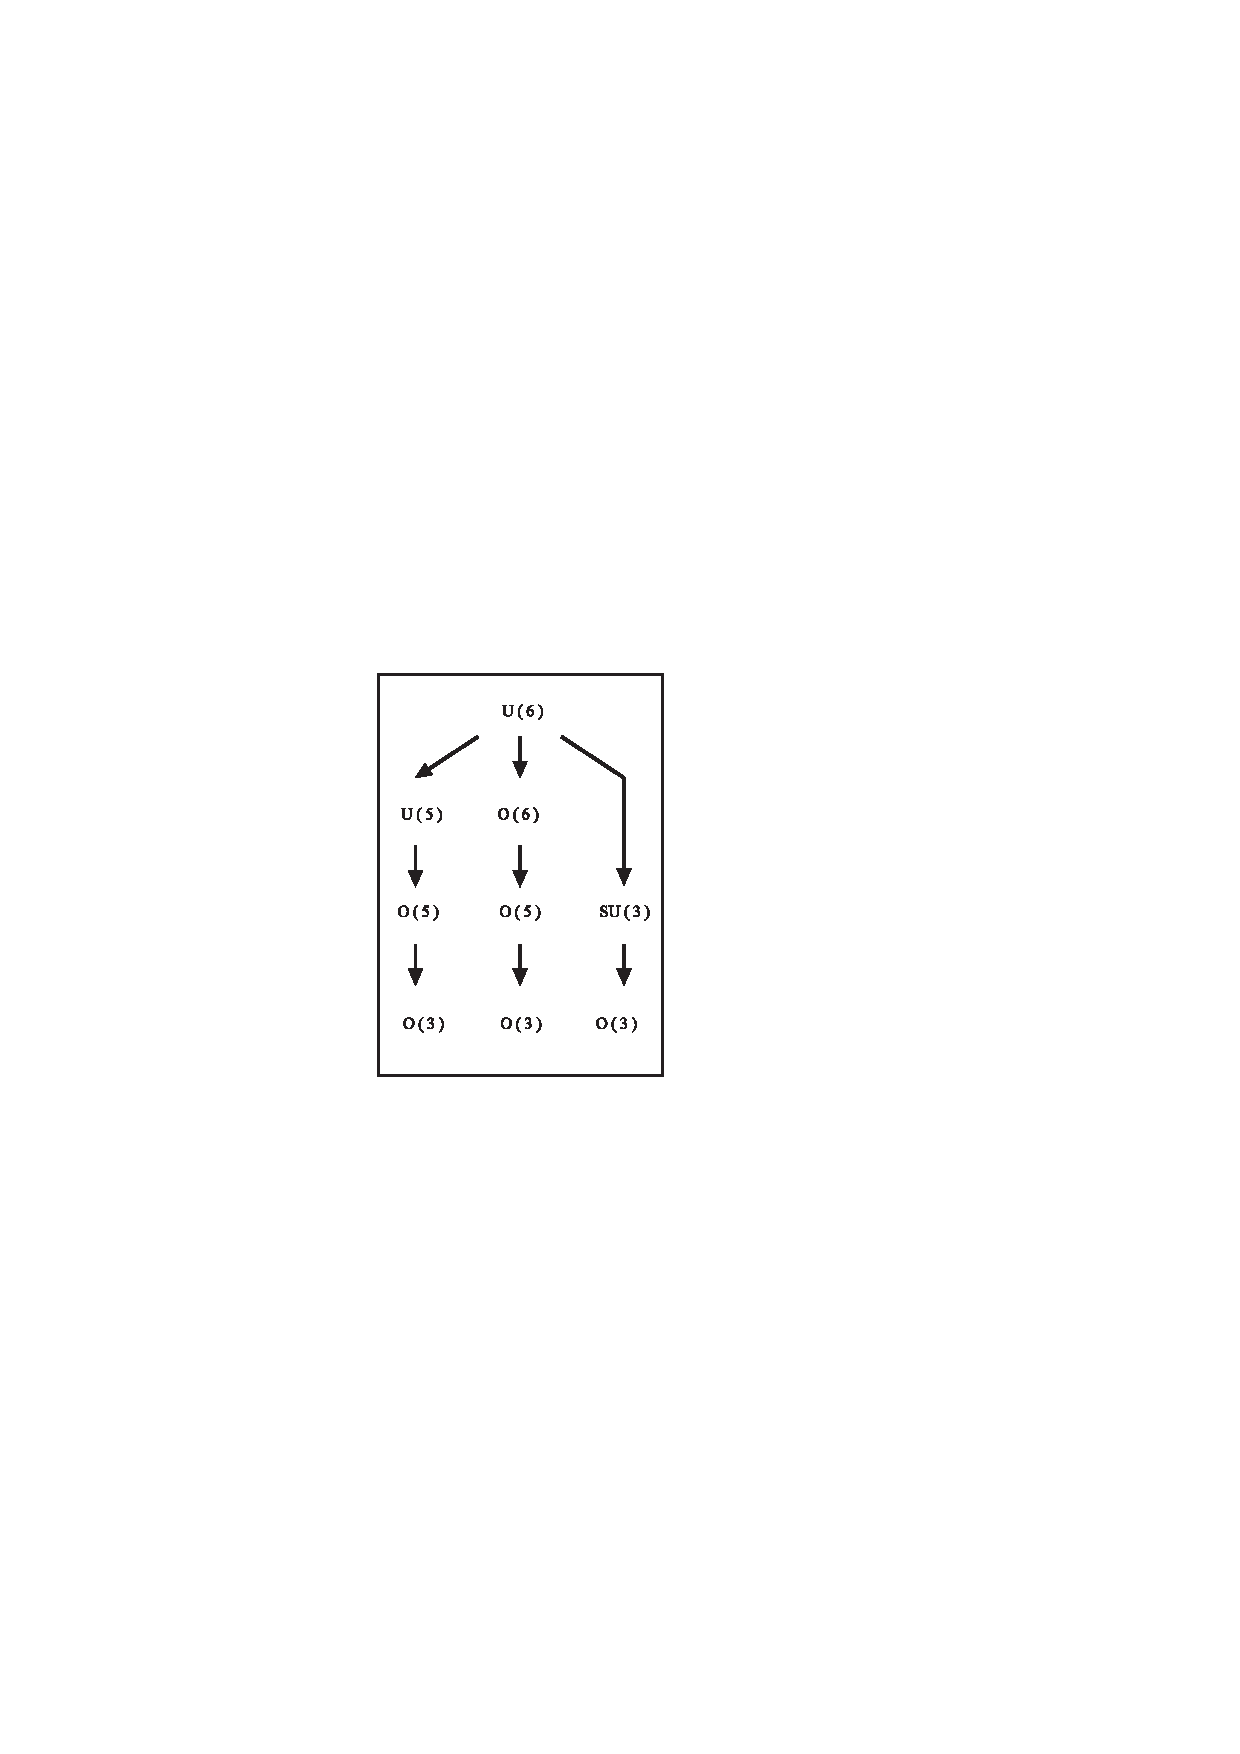
\includegraphics{tex_files/figs/authorfig1.jpeg}
\end{minipage}
\caption{Titlu comun, dar trebuie explicat ce e 'in st\^anga 'si ce e 'in dreapta.}
\label{fig:figura_exemplu2}       
\end{figure}

\begin{figure}[ht]  %preferinte: mai intai h - here apoi t- top, htb-, b-bottom
\begin{minipage}{0.5\textwidth}
\centering
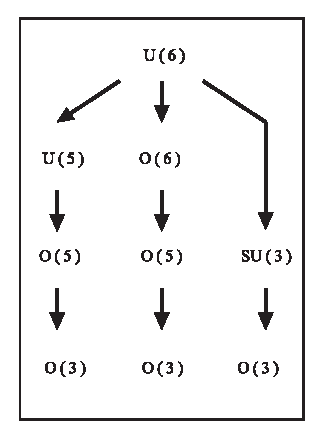
\includegraphics{tex_files/figs/authorfig1.eps}
%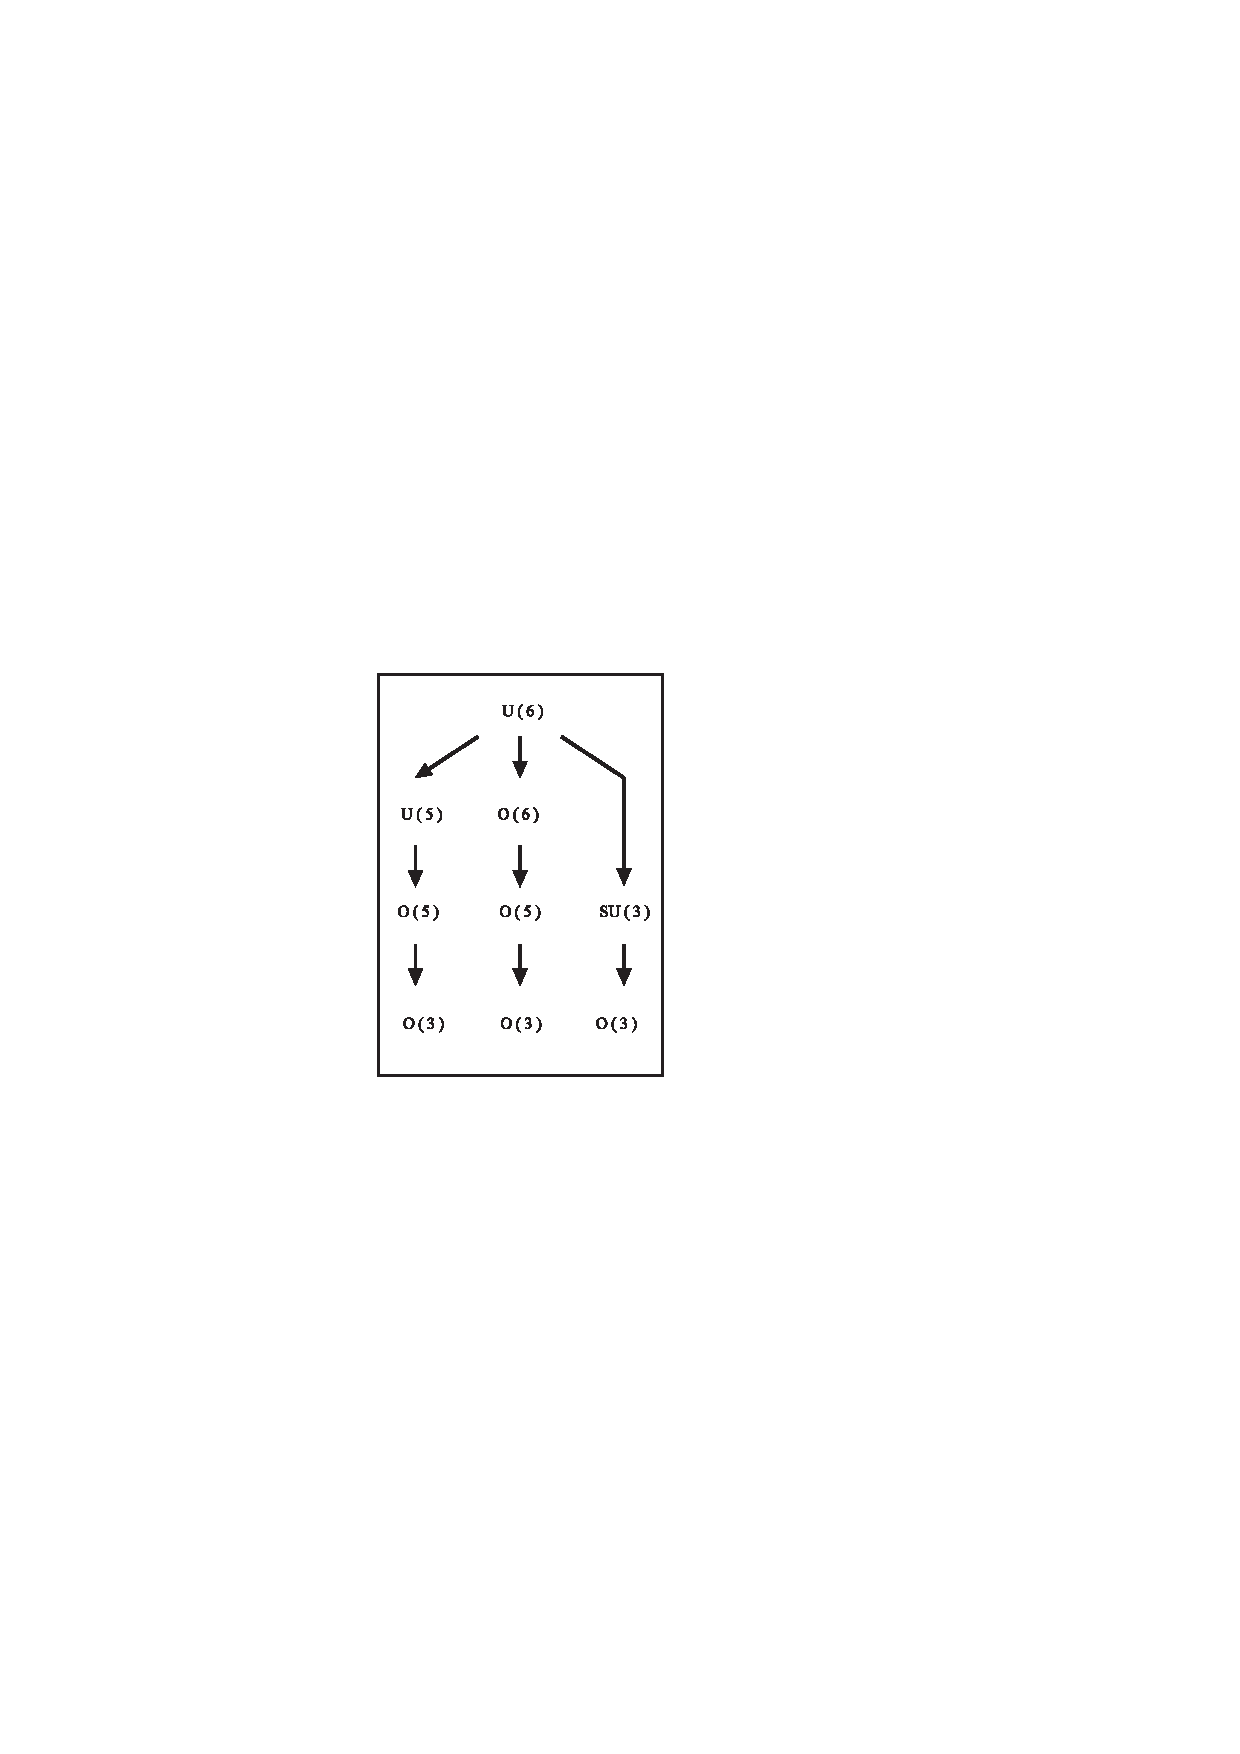
\includegraphics{tex_files/figs/authorfig1.jpeg}
\caption{Titlu st\^anga.}
\label{fig:figura_exemplu3}       
\end{minipage}
\begin{minipage}{0.5\textwidth}
\centering
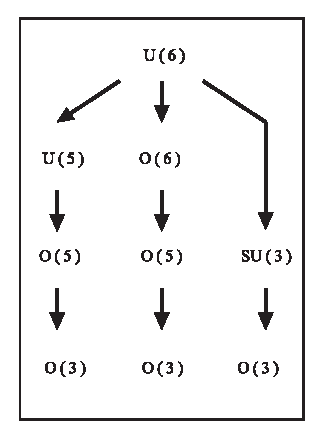
\includegraphics{tex_files/figs/authorfig1.eps}
%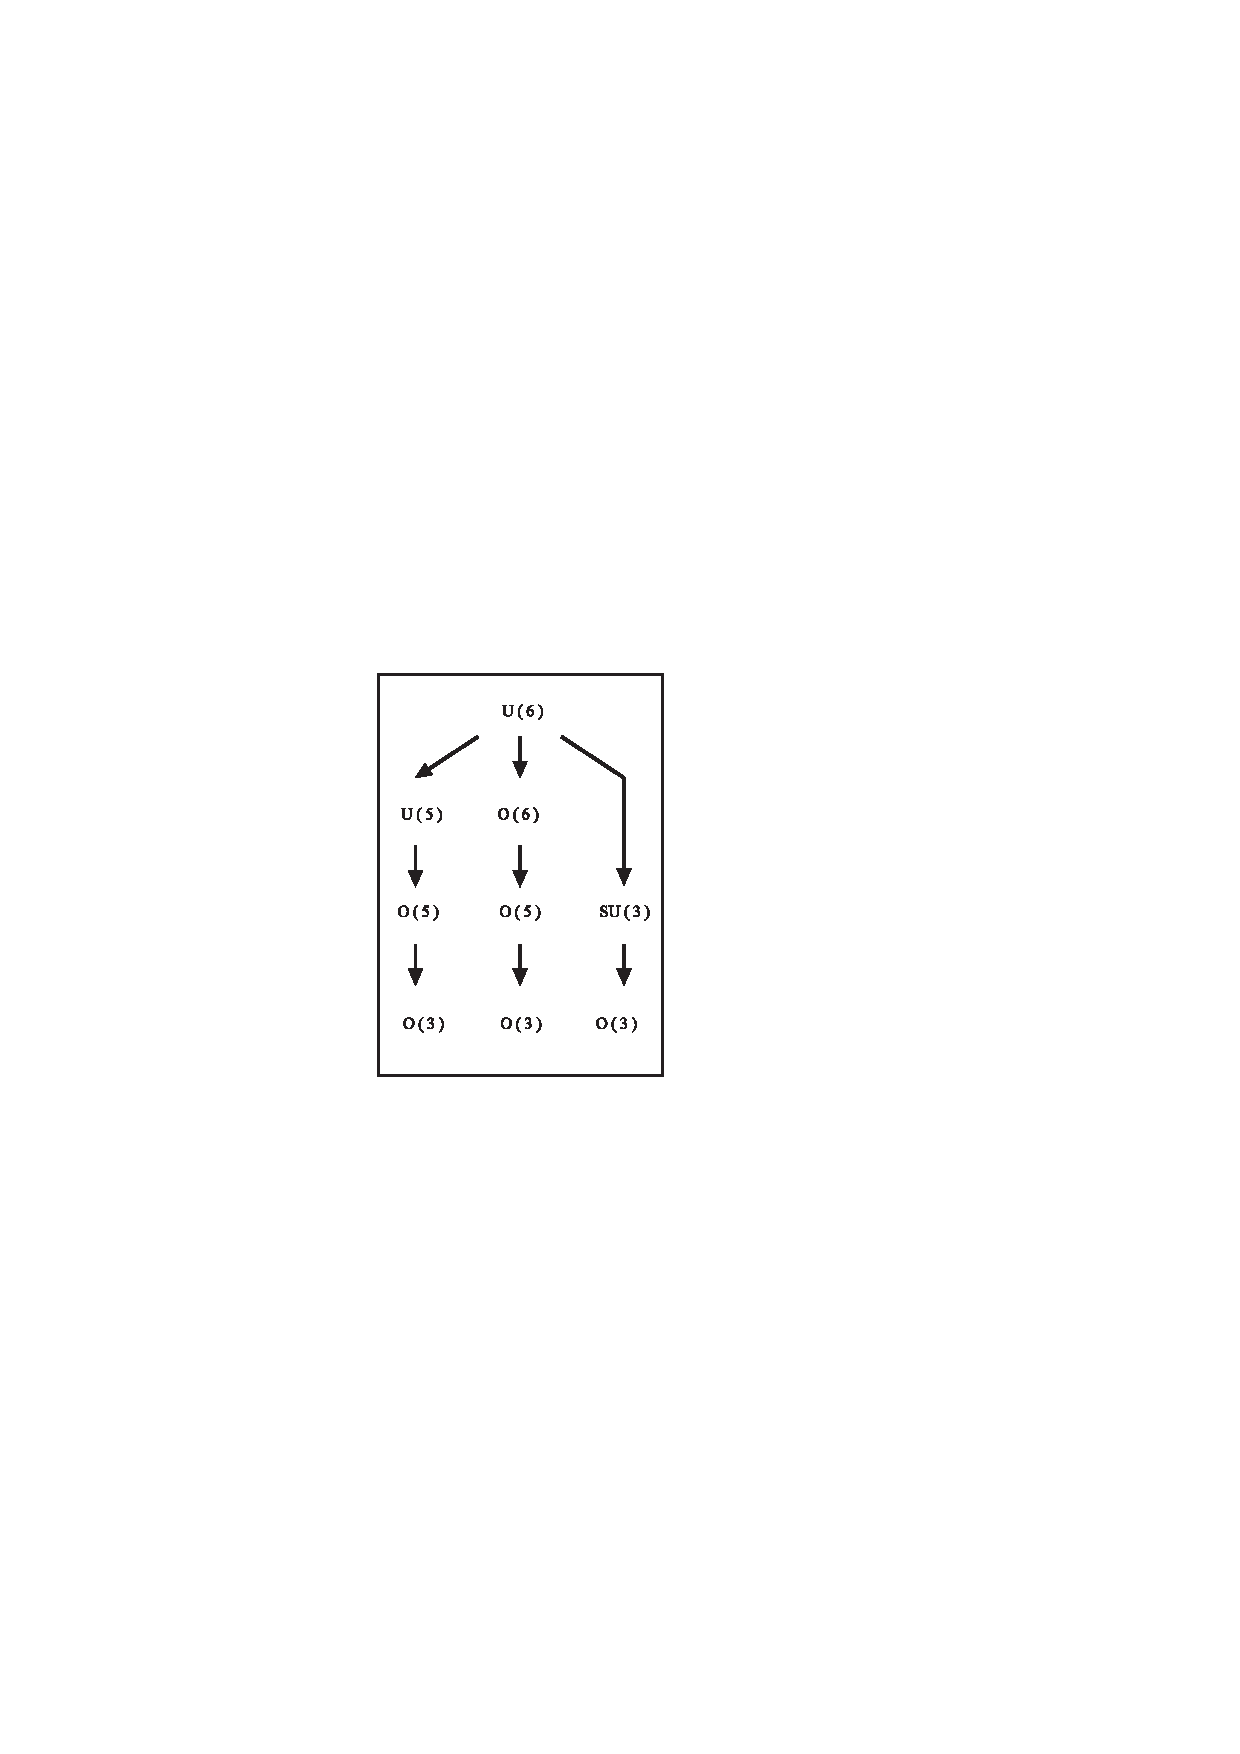
\includegraphics{tex_files/figs/authorfig1.jpeg}
\caption{Titlu dreapta.}
\label{fig:figura_exemplu4}       
\end{minipage}

\end{figure}

Pot fi folosite diferite formate de figuri, vede'ti documenta'tia\footnote{'In acest raport figurile sunt {\tt .eps}, iar documentul pdf a fost generat trec\^and prin formatul {\tt .ps}. 
'In Windows se poate folosi ca mediul de lucru TeXnicCenter 
\href{http://www.texniccenter.org/}{http://www.texniccenter.org/}, iar sub Linux, texstudio \href{http://www.texstudio.org/}{http://www.texstudio.org/}. 
Pentru lucrul sub linux pute'ti g'asi util fi'sierul {\tt Makefile} pe care 'il g'asi'ti de asemenea 'in arhiva de fi'siere. Citi'ti 'si observa'tiile din fi'sierul {\tt README1.txt}}.

Pentru figuri de calitate bun'a, este bine s'a folosi'ti imagini vectoriale \\ % rand liber fortat pentru ca link-ul e prea lung 
\href{http://www.techterms.com/definition/vectorgraphic}{http://www.techterms.com/definition/vectorgraphic}.

S-ar putea uneori s'a dori'ti s'a realiza'ti o figur'a de calitate mai bun'a prin folosirea unui limbaj, vede'ti de exemplu
\href{https://en.wikipedia.org/wiki/PGF/TikZ}{https://en.wikipedia.org/wiki/PGF/TikZ}.
Un exemplu de astfel de figur'a este 
Fig.\ref{fig:tikz}. Figura este preluat'a de la \\
\href{http://tex.stackexchange.com/questions/158668/nice-scientific-pictures-show-off}{http://tex.stackexchange.com/questions/158668/nice-scientific-pictures-show-off}.

\begin{figure}[ht]  %preferinte: mai intai h - here apoi t- top, htb-, b-bottom
\centering
%% Generated with LaTeXDraw 2.0.8
% Tue Nov 02 10:50:27 EET 2010
% \usepackage[usenames,dvipsnames]{pstricks}
% \usepackage{epsfig}
% \usepackage{pst-grad} % For gradients
% \usepackage{pst-plot} % For axes
\scalebox{1} % Change this value to rescale the drawing.
{
\begin{pspicture}(0,-4.5892186)(13.021875,4.6092186)
\definecolor{colormyred}{rgb}{0.8,0.0,0.0}
\definecolor{colormygreen}{rgb}{0.2,0.6,0.0}
\definecolor{colormyblue}{rgb}{0.0,0.2,0.8} % albastru
\psline[linewidth=0.04cm,arrowsize=0.1cm 2.0,arrowlength=2,arrowinset=0.4]{->}(0.9,-0.32)(11,-0.32)
\psline[linewidth=0.04cm,arrowsize=0.1cm 2.0,arrowlength=2,arrowinset=0.4]{<-}(5.3,4.3)(5.3,-4.5)
\psline[linewidth=0.08cm,linecolor=colormygreen](0.0,-2.0892189)(12.34,4.0107813)
\psline[linewidth=0.08cm,linecolor=colormyred](2.46,-4.5692186)(11.7,4.5107813)
\psframe[linewidth=0.06,linecolor=colormyblue,linestyle=dashed,dash=0.16cm 0.16cm,dimen=outer](6.78,0.55078125)(5.3,-0.32)
\psframe[linewidth=0.06,linecolor=colormyblue,linestyle=dashed,dash=0.16cm 0.16cm,dimen=outer](7.66,1.2507813)(6.78,0.55078125)
\psframe[linewidth=0.06,linecolor=colormyblue,linestyle=dashed,dash=0.16cm 0.16cm,dimen=outer](8.4,1.7107812)(7.66,1.2507813)
\usefont{T1}{ptm}{m}{n}
\rput(11.1,0.02078125){$x_1$}
\usefont{T1}{ptm}{m}{n}
\rput(4.9414062,4.2407813){$x_2$}
\usefont{T1}{ptm}{m}{n}
\rput(10.651406,4.420781){\color{colormyred}$\Delta_1$}
\usefont{T1}{ptm}{m}{n}
\rput(12.241406,3.3807812){\color{colormygreen}$\Delta_2$}
\usefont{T1}{ptm}{m}{n}
\rput(5.8,0){${\mathbf{x}^{(0)}}$}
\usefont{T1}{ptm}{m}{n}
\rput(7.2,0.8){${\mathbf{x}^{(1)}}$}
%\usefont{T1}{ptm}{m}{n}
%\rput(8.7,2){${\mathbf{x}^{(2)}}$}
\end{pspicture} 
}
  % trebuie sa compilati prin postscript
  \begin{tikzpicture}

\draw[thick,-latex] (0,0,0) -- (4,0,0) node[anchor=north east]{$y$};
\draw[thick,-latex] (0,0,0) -- (0,7.5,0) node[anchor=north west]{$z$};
\draw[thick,-latex] (0,0,0) -- (0,0,5) node[anchor=south]{$x$};
\filldraw (0,6,0) circle (1.75pt) node[left,font=\small]{$P(0,0,b)$};

\fill[top color=gray!50!black,bottom color=blue!10,middle color=gray,shading=axis,opacity=0.25] (0,0) circle (2cm and 0.5cm);
\fill[left color=gray!50!black,right color=blue!50!black,middle color=gray!50,shading=axis,opacity=0.25] (2,0) -- (2,4) arc (360:180:2cm and 0.5cm) -- (-2,0) arc (180:360:2cm and 0.5cm);
\fill[top color=blue!90!,bottom color=blue!2,middle color=blue!30,shading=axis,opacity=0.25] (0,4) circle (2cm and 0.5cm);
\draw (-2,4) -- (-2,0) arc (180:360:2cm and 0.5cm) -- (2,4) ++ (-2,0) circle (2cm and 0.5cm);
\draw[densely dashed] (-2,0) arc (180:0:2cm and 0.5cm);

\draw[densely dashed] (-2,2.8) arc (180:0:2cm and 0.5cm);
\draw[densely dashed] (-2,2.6) arc (180:0:2cm and 0.5cm);
\draw[thick] (-2,2.8) arc (180:360:2cm and 0.5cm);
\draw[thick] (-2,2.6) arc (180:360:2cm and 0.5cm);
\draw[thick, orange] (2,2.6) -- (3,2.6);
\draw[thick, orange] (2,2.8) -- (3,2.8);
\draw[thick,-latex] (2.8,4) -- (2.8,2.8);
\draw[thick,-latex] (2.8,1.6) -- (2.8,2.6);
\draw[thick,latex-] (2.8,0) -- (2.8,1.2) node[above] {$z$};
\draw [dashed] (0,6)--(3,6);
\draw[thick,latex-] (2.8,6) -- (2.8,4.5)node[below]{$b-z$};
\node at (3.5,2.7) [anchor=east]{$dz$};
\node at (2,1.5) [anchor=east]{$\rho_v\ (C/m^3)$};
\draw (-2,0) to[dim above=$L$,color=orange] (-2,4) ;

\coordinate (vec1) at (30:1);
\draw[-latex,thick] (0,0) -- (vec1)node[midway,sloped, above, inner sep=1] {$a$};
\draw[ultra thick,-latex,blue] (0,6,0) -- (0,7,0) node[right] {$\mathbf{E}$};
     \end{tikzpicture}   
\caption{Figura generat'a cu comenzi Tikz}
\label{fig:tikz}
\end{figure}

\subsubsection{Tabele}

Informa'tia de tip tabelar, trebuie prezentat'a ca 'in
Tabelul~\ref{tab:exemplu_tabel}.

\begin{table}[ht]  %preferinte: mai intai h - here apoi t- top, htb-, b-bottom
\centering
\caption{Titlurile tabelelor se pun deasupra tabelelor.}
\label{tab:exemplu_tabel}       % eticheta trebuie sa fie unica
%
% Informatia propriu zisa urmeaza
%
\begin{tabular}{|p{2cm}||c|l|r|p{3cm}|}  \hline  % l = left, c = center, r = right
Metoda & Dimensiune $n$ & Info1 & Info2 &Obs.  \\ \hline \hline
Metoda A & $10^3$  & 22 (19--25) & AAA& aaa\\
Metoda B & $3 \cdot 10^{4}$ & 21 & BB & bb\\
Metoda C & $10^6$  & 21--22 & CCCC& ccccc\\  \hline
\end{tabular}
\end{table}

\subsubsection{Liste}

Pentru listele numerotate se folose'ste \verb|enumerate|
ca de exemplu:
\begin{enumerate}
\item{Text aaa.}
\begin{enumerate}
\item{Text bbb.}
\item{Text ccc.}
\end{enumerate}
\item{Text ddd.}
\end{enumerate}

Pentru listele nenumerotate se folose'ste \verb|itemize| ca de exemplu:
\begin{itemize}
\item{Text 'in list'a nenumerotat'a, referire la Tabelul~\ref{tab:exemplu_tabel}.}
\begin{itemize}
\item{Text 'in list'a nenumerotat'a - x.}
\item{Text 'in list'a nenumerotat'a - y.}
\end{itemize}
\item{Text 'in list'a nenumerotat'a - z.}
\end{itemize}

Pentru o list'a de defini'tii sau nota'tii pute'ti folosi \verb|description|, ca de exemplu
\begin{description}
\item[$\vect{E}$]{Intensitatea c\^ampului electric [V/m] - m'arime fizic'a vectorial'a, ce caracterizeaz'a local starea c\^ampului electric 'in vid. }
\item[$\vect{H}$]{Intensitatea c\^ampului magnetic [A/m] - m'arime fizic'a vectorial'a, ce caracterizeaz'a local starea c\^ampului magnetic 'in vid. }
\end{description}



\subsubsection{Anima'tii}

\LaTeX \, nu poate include gif-uri animate. Se pot crea 'ins'a anima'tii pe baza unor frame-uri salvate 'in prealabil. 

%Dac'a ve'ti compila f'ar'a a trece prin  format postscript atunci pot fi folosite (printre altele) frame-uri 'in format {\tt.png}, {\tt.jpg}. Dac'a trece'ti prin postscript (obligatoriu dac'a ave'ti figuri create cu {\tt{pstricks}}), atunci frame-urile trebuie s'a fie 'in format {\tt{.eps}}.

Pentru a include anima'tii 'in \LaTeX, trebuie s'a folosi'ti pachetul {\tt{animate}} care poate fi desc'arcat de la \href{https://www.ctan.org/tex-archive/macros/latex/contrib/animate?lang=en}{www.ctan.org}. 
\begin{verbatim}
\usepackage{animate}
\end{verbatim}
Comanda de utilizare este
\begin{verbatim}
\animategraphics[<options>]{<frame rate>}{<file basename>}{<first>}{<last>}
\end{verbatim}
Spre exemplu, pentru a crea o anima'tie din figurile salvate 'in frame-urile {\tt{frame0.png}}, {\tt{frame1.png}}, {\tt{frame2.png}}, {\tt{frame3.png}}, scalate la 50\% din dimensiunea ini'tial'a a imaginilor, derulate la infinit, c\^ate 5 frame-uri pe secund'a, comanda este:
\begin{verbatim}
\animategraphics[loop,autoplay,scale=0.5]{5}{frame}{0}{3}
\end{verbatim}


%\begin{figure}[b]
%\begin{center}
%%%%%\includegraphics{tex_files/matlab_animate/frame_0.eps}
%\animategraphics[label=animfun,loop,autoplay,scale=0.4]{4}{tex_files/matlab_animate/frame_}{0}{15}
%\mediabutton[
%    jsaction={
%      if(anim['animfun'].isPlaying)
%        anim['animfun'].pause();
%      else  
%        anim['animfun'].playFwd();
%    }
%  ]{\fbox{Play/Pause}}
%\caption{Exemplu de anima'tie. Frame-urile au fost create 'in Matlab.}
%\label{fig:animatie}
%\end{center}
%\end{figure}



%Exist'a metode diverse de a genera frame-urile. 'In Fig.\ref{fig:animatie} observa'ti o astfel de anima'tie 'in care frame-urile au fost create 'in {\tt{Matlab}}. Dac'a a'ti creat un gif cu un alt instrument, atunci o variant'a de a-l transorma 'in frame-uri este cea online, disponibil'a la {\href{http://toolson.net/GifResizer}{toolson}}

\subsubsection{Circuite electrice}

Pute'ti desena circuite cu ajutorul pachetul circuitiks,
disponibil la\\ \href{https://www.ctan.org/pkg/circuitikz}{https://www.ctan.org/pkg/circuitikz}

'In Fig.\ref{fig:circuit1} ave'ti un exemplu de astfel de schem'a, 'in care sunt folosite simboluri IEEE.
\begin{figure}[b]
\begin{center}
 \begin{circuitikz}[scale=1.4,american]\draw
 (0,0) to[C, l=10<\micro\farad>] (0,2) -- (0,3)
 to[R, l=2.2<\kilo\ohm>] (4,3) -- (4,2);
 \draw (4,0) to[L, l_=12<\milli\henry>, i<_=$i_1$] (4,2);
 \draw (4,0) -- (0,0)
 (4,2) { to[D*, *-*, color=red] (2,0) }
 (0,2) to[R, l=1<\kilo\ohm>, *-] (2,2)
 to[V, i_=$i_2$,v^=$e(t)$] (4,2)
 (2,0) to[I, l=$j(t)$, -*] (2,2)
  ;\end{circuitikz}
  \caption{Circuit realizat cu circuitiks, simboluri "americane".}
  \label{fig:circuit1}
  \end{center}
  \end{figure}

Dac'a dori'ti s'a folosi'ti simboluri ca 'in c'ar'tile clasice scrise 'in limba
rom\^an'a, atunci pute'ti adauga pachetului circuitiks simbolurile create de Adrian Pop,
disponibile la
\href{https://github.com/PopAdi/circuitikz-romanian-symbols}{https://github.com/PopAdi/circuitikz-romanian-symbols}.

Acela'si circuit, desenat cu astfel de simboluri, este cel din
Fig.\ref{fig:circuit2}.

\begin{figure}
\begin{center}
\begin{circuitikz}[scale=1.4,european resistors,american inductors]\draw
(0,0) to[C, l=10<\micro\farad>] (0,2) -- (0,3)
to[R, l=2.2<\kilo\ohm>] (4,3) -- (4,2);
\draw (4,0) to[L, l_=12<\milli\henry>, i<_=$i_1$,v^=$u_1$] (4,2);
\draw (4,0) -- (0,0)
(4,2) { to[D*, *-*, color=red] (2,0) }
(0,2) to[R, l=1<\kilo\ohm>, *-] (2,2)
to[romanianVoltageSource, i_=$i_2$,v^=$e(t)$] (4,2)
(2,0) to[romanianCurrentSource, l=$j(t)$, -*] (2,2)
 ;\end{circuitikz}
 \caption{Circuit realizat cu circuitiks, simboluri utilizate 'in c'ar'ti clasice 'in limba rom\^an'a.}
   \label{fig:circuit2}
   \end{center}
   \end{figure}

 
\section{Alte exemple 'si idei}

Un rezultat interesant este dat de
\begin{equation}
\label{eq:camp}
\vect{E}(\vect{r}) = \vect{E}_0 \eul^{\I\vect{k}\cdot\vect{r}},  %\vect, \eul si \I au fost definiti in preambul
\end{equation}
unde $\vect{E}$ este intensitatea c\^ampului electric, $\vect{r}$ este vectorul de pozi'tie, $\vect{k}$ este num'arul de und'a vectorial, iar
$\vect{E}_0$ este intensitatea c\^ampului electric 'in origine.

Observa'ti cum sunt puse semnele de punctua'tie 'in toat'a fraza anterioar'a.

\subsection{Pagina de titlu}

Dac'a folosi'ti stilul {\tt report} 'si nu stilul {\tt article} ca 'in acest document\footnote{Pentru rapoarte mai mari cum sunt cele de licen't'a sau de dizerta'tie, atunci stilul {\tt report} este mai potrivit. Pentru teme de cas'a 'si rapoarte scurte, atunci este mai potricit stiul {\tt article}.}, atunci titlul este scris separat pe prima pagina. 
'In acest caz pute'ti realiza o prim'a pagin'a cu un aspect mai frumos, iar machete pentru astfel de prime pagini 
g'asi'ti de exemplu la \\  % fortare la rand nou pentru ca link-ul e prea mare si iese din pagina
\href{http://www.latextemplates.com/cat/title-pages}{http://www.latextemplates.com/cat/title-pages}.

\subsection{Pseudocoduri}

Dac'a ave'ti de scris pseudocoduri, pute'ti proceda cum este descris de exemplu la \\
\href{http://en.wikibooks.org/wiki/LaTeX/Algorithms}{http://en.wikibooks.org/wiki/LaTeX/Algorithms}.


\subsection{Prezent'ari}

Dup'a ce a'ti scris un raport 'in \LaTeX\, evident c'a prezentarea se face natural tot 'in \LaTeX\, numai c'a trebuie s'a folosi'ti un stil potrivit.

Un exemplu posibil este stilul \texttt{beamer}, detalii g'asi'ti aici \\
\href{http://en.wikipedia.org/wiki/Beamer_(LaTeX)}{http://en.wikipedia.org/wiki/Beamer\_(LaTeX)}.

Iat'a dou'a exemple, realizate cu dou'a stiluri implicite ale pachetului \texttt{beamer}. 

\href{http://an.lmn.pub.ro/slides2014/AN_Erori_2014.pdf}{http://an.lmn.pub.ro/slides2014/AN\_Erori\_2014.pdf}

\href{http://an.lmn.pub.ro/slides2014/AN_MetodeDirecte_2_2014.pdf}{http://an.lmn.pub.ro/slides2014/AN\_MetodeDirecte\_2\_2014.pdf}


\section{Fi'siere .bib. Bibtex.}

Organiza'ti-v'a referin'tele 'in fi'siere \texttt{.bib}, iar referin'tele crea'ti-le
cu comanda \verb \cite. Folosi'ti \texttt{bibtex} pentru generarea automat'a a referin'telor.

Cit'arile se fac 'in text, 'in stilul urm'ator.

Dou'a c'ar'ti celebre sunt \cite{golub:96,Cormen:90}, iar un raport excelent este \cite{Shewchuk:94}. Referin'ta \cite{ciuprina:atee11}
este un articol de conferin't'a. Pentru lucr'ari care au un num'ar mare de referin'te se recomand'a folosirea stilului \texttt{alpha} 'si nu
\texttt{plain}.

De multe ori, dac'a o lucrare pe care vre'ti s'a o cita'ti o g'asi'ti pe internet, s-ar putea s'a g'asi'ti 'si liniile de text necesare unei intr'ari bibliografice pentru \texttt{bibtex}. Mergeti de exemplu la
\href{http://ieeexplore.ieee.org/Xplore/home.jsp}{http://ieeexplore.ieee.org/Xplore/home.jsp}, alegeti un articol oarecare, de exemplu
\href{http://ieeexplore.ieee.org/xpl/articleDetails.jsp?arnumber=6842585}{http://ieeexplore.ieee.org/xpl/articleDetails.jsp?arnumber=6842585}  'si apoi observa'ti c'a pute'ti alege {\tt Download} apoi {\tt Citations}, apoi {\tt Bibtex}. Rezultatul este
\begin{small}
\begin{verbatim}
@ARTICLE{6842585, 
author={Han Hu and Yonggang Wen and Tat-Seng Chua and Xuelong Li}, 
journal={Access, IEEE}, 
title={Toward Scalable Systems for Big Data Analytics: A Technology Tutorial}, 
year={2014}, 
month={}, 
volume={2}, 
pages={652-687}, 
ISSN={2169-3536},}
\end{verbatim}
\end{small}

Alternativ, pute'ti scrie bibliografia 'intr-un fi'sier, 'intre 
\begin{verbatim}
\begin{thebiliography}
.....
\end{thebibliography}
\end{verbatim}
'In acest caz nu ave'ti niciun fel de flexibilitate 'in organizarea
'si formatarea referin'telor. 

\section{Informa'tii de detaliu}

Informa'tiile de detaliu se pun 'in anexe. De exemplu, 'in anexa \ref{sec:preambul} g'asiti preambulul folosit pentru generarea acestui document, iar 'in anexa \ref{sec:codMatlab} g'asi'ti un cod Matlab.

\section{Cum trebuie s'a arate un raport 'stiin'tific}

Este bine s'a citi'ti sfaturi despre cum trebui redactate rapoartele 'stiin'tifice. Iat'a doar un exemplu
\href{http://writing.wisc.edu/Handbook/ScienceReport.html}{http://writing.wisc.edu/Handbook/ScienceReport.html}
dar desigur pute'ti g'asi 'si altele.

Iat'a de exemplu lucr'ari de dizerta'tie (prima este din USA, cealalta din Turcia):\\
\href{https://www.mri.psu.edu/faculty/stm/Student theses/A. Dogan.pdf}{https://www.mri.psu.edu/faculty/stm/Student\%20theses/A.\%20Dogan.pdf}\\
\href{http://etd.lib.metu.edu.tr/upload/1124676/index.pdf}{http://etd.lib.metu.edu.tr/upload/1124676/index.pdf}

\section{Concluzii} 

'Intotdeauna 'incheia'ti cu un paragraf special dedicat concluziilor.


\section*{Mul'tumiri}  % steluta inseamna faptul ca aceasta sectiune nu va aparea la cuprins

'In cazul 'in care raportul reprezint'a o lucrare mai ampl'a sau un articol 'stiin'tific, nu uita'ti s'a mul'tumi'ti pentru sprijinul financiar sau spiritual pe care l-a'ti primit. Pentru o lucrare de tip articol mul'tumirile se pun la sf\^ar'sit, ca aici. La o lucrare mai ampl'a, de tip raport, mul'tumirile se scriu la 'inceput, pe o pagin'a separat'a, 'inainte de cuprins.

Autoarea acestui document 'si a pachetului de fi'siere asociat lui mul'tume'ste urm'atorilor studen'ti\footnote{Lista este deschis'a $\ddot\smile$.} care au sugerat corec'tii 'si 'imbun'at'a'tiri: Adrian Pop, Adina Budriga, Denisa Sandu, Radu Stoichi'toiu, R'azvan Chi'tu, Darius Nea'tu, Daniel-Andrei Barbu.






  % fisierul principal nu include textul propriu-zis al documentului

\newpage % bibliografia sa inceapa pe pagina noua

%%%%%%%%% bibliografie
%\bibliographystyle{plain}   % in ordinea citarii, fisier de stil al distributiei standard Latex
\bibliographystyle{plainrom} % in ordinea citarii dar apare cuvanul "si" in loc de "and" intre autori - vedeti fisierul plainrom.bst
%\bibliographystyle{alpha}  % referinte sortate in ordine alfabetica, cu etichete alfanumerica - util pentru rapoarte mari
\addcontentsline{toc}{section}{Bibliografie}  % adauga linia "Bibliografie" la table of contents
\bibliography{referinte_exemplu}  % in pachetul de fisiere exista fisierul referinte_exemplu.bib

\newpage
\begin{appendix}
\section{Preambul folosit pentru generarea acestui document}
\label{sec:preambul}

Preambulul folosit pentru generarea acestui document este urm'atorul:

\begin{small}
\begin{verbatim}
\documentclass[12pt,twoside]{article}  
\usepackage{amsmath,epsfig,pifont,calc,pifont,pstricks}
\usepackage{media9}
\usepackage{animate} % daca includeti animatii
\usepackage{graphicx}	
\usepackage[romanian]{babel}
\usepackage[unicode]{hyperref} 
\usepackage{rom} 		 % pentru a scrie cu diacritice in limba romana	

%%% setari ale paginii
\setlength{\parindent}{3ex}
%dimensiunea textului pe pagina
\setlength{\voffset}{-2cm}
\setlength{\textheight}{23cm}  
\setlength{\textwidth}{16cm}
\setlength{\topmargin}{0cm}
\setlength{\headsep}{1cm}
\renewcommand{\baselinestretch}{1.2}
\newcommand{\myindent}{\hspace*{3ex}}
%\renewcommand{\baselinestretch}{1}

%margini
\setlength{\oddsidemargin}{0.5cm}
\setlength{\evensidemargin}{-0.3cm}
%\raggedright
\raggedbottom

%% - macro-uri definite de autor
\newcommand{\D}{\mathrm{d}}	% va fi folosita in mediul matematic, 
                            % pentru diferentiala d
\newcommand{\I}{\mathrm{i}}	% va fi folosita in mediul matematic, 
                            % pentru unitatea imaginara
\newcommand{\eul}{\mathrm{e}}	% numarul lui Euler
\newcommand{\vect}[1]{\mathbf{#1}}	% comanda cu un argument, 
                            % pentru scrierea vectorilor cu lidere aldine, drepte
                            % comanda \vec a LaTeX pune sageti deasupra.
																										
\newcommand{\reale}{\mbox{${\scriptstyle \rm I\!R}$}}  % multimea numerelor reale
\newcommand{\complexe}{\mbox{${\scriptstyle \rm I\!\!\!\!C}$}}
\newcommand{\rationale}{\mbox{${\scriptstyle \rm I\!\!\!\!Q}$}}
\newcommand{\naturale}{\mbox{${\scriptstyle \rm I\!\!N}$}}
\newcommand{\intregi}{\mbox{${\scriptstyle \rm Z\!\!\!Z}$}}
%% end preambul
\end{verbatim}
\end{small}

\section{Cod Matlab}
\label{sec:codMatlab}

Acesta este un cod matlab. Pute'ti descoperi 'si singuri ce face.

\lstinputlisting{tex_files/cod/codMatlab.m}

\end{appendix}

\end{document}
